\chapter{HIL felépítése}

\todo

\section{Hardware felépítése}

A HIL szimulátor hardware nem más, mint egy interface elektronika a vezérlő hardware-ek és a szimulációt végző FPGA között. \Afigref{hw_architect} ábrán láthatóak a vezérést végző elemek. A HIL szimulátor feladata a bal oldali, Power Subsystemb blokkból érkező jelek előállítása, illetve a vezérlő jelek fogadása. Mivel a szimuláció során a PIB nem szükséges, ezért az MCB és a CCB kapcsolatát is a HIL elektronika biztosítja.

\todo[inline]{Blokkvázlat a HIL-ről}

\subsection{Tápegység}
A kártya $24 V$-os tápfeszültségre lett tervezve. Ebből egy Linear Technologies \emph{LT3845AEFE#PBF} szinkron buck tápegység vezérlő IC és a hozzá tartozó külső apparátus állítja aelő az $5 V$-os tápfeszültséget mind az FPGA mind pedig a CCB számára. A tápegység maximálisan $6 A$ terhelhetőségű, amely előser soknak tűnhet, de az FPGA fogyasztását jelentpsen befolyásolja a benne található firmware, így elképzelhető az kapacitás teljes felhasználása is, kis teljesítmény esetén edig hatékony tud maradni az ún. \emph{Burst mode} működési mód segítségével.

\subsecton{Szigma-Delta átalakítók}

Az FPGA nem rendelkezik analóg kiementekkl, azonban a CCB számára elő kell állítani a normál működés során visszamért analóg jeleket, hiszen ebben relik a szimulátor lényege, a vezérlő elektronika szmszögéből nincsen különbség a valós hardware és a szimulátor között. 

\subsection{ZTEX kártya}

Egy iylen teszt és fejlesztési eszköz fejlesztése során az egiyk legfontosabb szempont a modularitás. Nem láthatjuk előre feltétlenül, hogy a későbbiekben mire lesz szükség. Az FPGA önmagában biztosít modularitást, hiszen cserélhető benne a hardware, jelen esetben a megvalósított matematikai modell. Ezen felül egy közel 500 lábbal rendelkező BGA tokos FPGA-hoz a nyáktervezés sem triviális feladat. A megfelelő lábak kivezetéséhez legalább 6-8 rétegre van szükség, és nagyon sok hibalehetőséget tartogat magában. Ezek miatt egy FPGA modul alkalmazása mellett döntöttünk. Bár az elérhető GPIO lábak mennyisége így korlátoztt, az FPGA-t működtető áramkör garantáltan működőképes, illetve a saját tervezésű elektornika bonyolultsága is jelentősen csökken.

\begin{figure}[!ht]
	\centering
	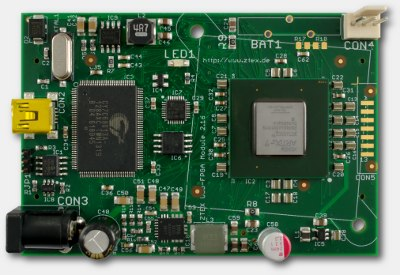
\includegraphics[width = \textwidth]{figures/fpga216.jpg}
	\caption{A ZTEX 2.16 FPGA board} 
	\label{fig:ztex}
\end{figure}

\Aref{fig:ztex} ábrán látható ZTEX panel mellett tettem le a voksom. A kártyán található egy USB-s loader, így JTAG programozó eszköz sem feltétlenül szükséges az FPGA feltöltéséshez, illetve FLASH memória is található az eszközön, így automatikusan minden indulákor betöltődik a firmware az FPGA-ba.


\begin{figure}[!ht]
	\centering
	\includegraphics[width = \textwidth]{figures/fpga216blox.jpg}
	\caption{A ZTEX 2.16 FPGA board felépítése} 
	\label{fig:ztex_block}
\end{figure}

\todo[inline]{Képhiba}

Ezen felül a rajta található Xilinx Artix 7 FPGA megfelelő hűtését is biztosítja a panel. Az FPGA főbb datai \aref{table:artix7spec} táblázatban láthatóak. Ez az eszköz a Xilinx jelegelg kereskedelemi forgalomban kapható egyik zászlóshajója, amit bizonyít is a ZTEX panel 500 Eurós vételára.

\begin{table}[]
\centering
\begin{tabular}{ll}
Logikai cellák               & 215360 \\
Szeletek                     & 33650  \\
CLB Flip-flopok              & 269200 \\
Eloszott memória (kb)        & 2888   \\
Blokk RAM/FIFO (36 kb/darab) & 365    \\
Blokk RAM összesen (kb)      & 13140  \\
                             &        \\
                             &        \\
                             & 
\caption{A Xilinx Artix 7 XC7A200T}
\label{artix7spec}      
\end{tabular}
\end{table}



\section{A szimulátor szerepe a folyamatban}
\section{A szimulátor felépítése}
\subsection{A hardware felépításe}
\subsection{A firmware felépítése}